\documentclass[conference]{IEEEtran}
\IEEEoverridecommandlockouts
% The preceding line is only needed to identify funding in the first footnote. If that is unneeded, please comment it out.
\usepackage{cite}
\usepackage{amsmath,amssymb,amsfonts}
\usepackage{algorithmic}
\usepackage{graphicx}
\usepackage{textcomp}
\usepackage{xcolor}
\usepackage{booktabs}
\usepackage{float}
\usepackage{url}
\usepackage{multirow}
\usepackage{siunitx}

\def\BibTeX{{\rm B\kern-.05em{\sc i\kern-.025em b}\kern-.08em
    T\kern-.1667em\lower.7ex\hbox{E}\kern-.125emX}}

\graphicspath{{../results/}{../results/plots/}}

\begin{document}

\title{Topological Risk Analysis and Criticality Mapping in the NPM Supply Chain}

\author{\IEEEauthorblockN{1\textsuperscript{st} Yusuf Arbaç}
\IEEEauthorblockA{\textit{Dept. of Computer Engineering} \\
\textit{Fırat University}\\
Elazığ, Turkey \\
yusufarbac@firat.edu.tr}
}

\maketitle

\begin{abstract}
While centralized package managers like NPM accelerate software development by providing ready-to-use code libraries, the intricate web of nested dependencies among these components has transformed the ecosystem into a complex and fragile structure. Current security approaches remain insufficient in detecting these systemic risks, which stem from the network's structural architecture and possess the potential for cascading effects. This study aims to map systemic risks within the NPM ecosystem using topological analysis methods that are independent of package content. Within the scope of the analysis, a directed graph was constructed by modeling the top 1,000 packages with the most dependents in the NPM ecosystem, along with their dependencies extending up to a depth of 7. In-degree, out-degree, and betweenness metrics were calculated on the network, and a novel 'Composite Risk Score' (BRS) was developed through a weighted combination of these values. The statistical distribution of the calculated metrics reveals that the network exhibits a scale-free topology; consequently, risk is concentrated on a small number of critical nodes that form the backbone of the ecosystem. Robustness simulations confirmed that the removal of packages with high BRS scores leads to a destructive collapse in network integrity. This research contributes a novel topology-based perspective to the literature by emphasizing that limited security resources should be directed toward the critical nodes forming the ecosystem's backbone, rather than relying on random scans.
\end{abstract}

\begin{IEEEkeywords}
Software supply chain security, NPM, dependency network analysis, topological risk, cascade effect.
\end{IEEEkeywords}

\section{Introduction}
The pursuit of efficiency, a fundamental dynamic of modern software engineering, has made development processes dependent on ready-to-use code libraries provided by centralized package managers such as NPM, PyPI, and RubyGems \cite{wyss2025npm, duan2020measuring}. While this modular architecture accelerates software development, it has created a fragile foundation where a vulnerability at any point in the supply chain can spread to the entire ecosystem \cite{wyss2025npm}. The NPM ecosystem, hosting millions of packages and intricate dependency relationships between them, is an attractive target for threat actors due to its large attack surface \cite{wang2023threat}. The uncontrolled propagation of vulnerabilities through dependency networks \cite{liu2022demystifying, zerouali2022impact} and disruptions in package maintenance processes \cite{rahman2024update, cogo2020maintenance, jafari2023mitigation} increase this risk. The literature confirms that this network exhibits "small-world" characteristics, meaning a limited number of packages or maintainers have a disproportionate impact on the ecosystem \cite{zimmermann2019smallworld, hafner2021robustness, oldnall2017complex, jaisri2024selfcontained}.

Supply chain attacks manifest in a wide range, from the compromise of trusted packages to "typosquatting" traps where popular package names are mimicked \cite{ohm2020backstabber}. Source poisoning \cite{hastings2024poisoning}, prototype pollution \cite{shcherbakov2021prototype}, and dependency-based attacks specific to Node.js architecture \cite{yip2022dependency} reveal the diversity of threats. Comprehensive studies such as "Backstabber’s Knife Collection" \cite{ohm2020backstabber} and "The Hitchhiker’s Guide" \cite{ladisa2023hitchhiker} examine the anatomy of attacks through installation and runtime phases, while Duan et al. \cite{duan2020measuring} focus on registry-level exploits, documenting the existence of hundreds of malicious packages.

Against these threats, machine learning and dynamic analysis-based defense mechanisms like Amalfi \cite{sejfia2022amalfi}, Cerebro, and OSCAR \cite{zheng2024oscar} have been developed, as well as metadata analysis \cite{halder2024metadata}, malicious behavior sequences \cite{zhang2023behavior}, cross-language detection \cite{ladisa2023crosslang}, secure usage practices \cite{imtiaz2023secure}, and signature-based approaches \cite{correia2022detection, ohm2021acme, schorlemmer2024signing}. However, the massive scale of the ecosystem makes deep scanning of every package unsustainable in terms of cost and time.

There are valuable studies in the literature that analyze risk based on package maintenance status \cite{rahman2024update} or the propagation dynamics of known vulnerabilities \cite{liu2022demystifying}. However, approaches that measure systemic collapse risks (cascade effect) stemming from the network's topological structure and convert them into an operational risk score are limited. Existing studies generally reveal the general characteristics of the network at a descriptive level; they fall short in providing a concrete prioritization mechanism for the optimization of security resources. In this study, independent of package contents, the focus is solely on the topological architecture of inter-package dependencies, aiming to map structural risk.

Within the scope of the study, a directed graph constructed based on NPM's standard dependency resolution algorithms was used to develop a \textbf{Composite Risk Score (BRS)} by weighting in-degree, out-degree, and betweenness measurements. This model was supported by cascade effect and Largest Connected Component (LCC) analyses, revealing the systemic implications of topological risk with quantitative data. Thus, the aim is to direct limited security resources to the most critical points by creating a prioritized watch list for security analysts and package managers.

\section{Data and Method}

\subsection{Dataset Creation and Scope}
In this study, a sampling strategy centering on systemic impact rather than sheer download numbers was adopted. Accordingly, the top 1,000 packages with the most \textit{dependents} according to \texttt{ecosyste.ms} data were determined as the seed set, and all dependencies of this set up to the 7th depth level were included in the analysis. Following a data preprocessing stage where circular references were resolved, a directed graph consisting of 1,506 nodes and 3,058 edges was obtained. The Python NetworkX library was used for network modeling and analysis processes.

\subsection{Centrality Measures and Normalization}
Three centrality metrics were used to determine the importance of packages within the network:
\begin{itemize}
    \item \textbf{In-Degree:} Represents the number of directly dependent packages. It is an indicator of popularity and direct sphere of influence.
    \item \textbf{Out-Degree:} Shows the number of external dependencies. High out-degree indicates the breadth of the attack surface.
    \item \textbf{Betweenness:} The frequency of being on the shortest paths. It reflects the package's bridge role and strategic position in the network.
\end{itemize}

\subsection{Mathematical Model}
The NPM ecosystem is modeled as a directed graph $G=(V, E)$ where packages represent nodes ($V$) and dependencies represent edges ($E$). Before calculating the risk score for each node $v \in V$, metrics were normalized to the $[0,1]$ range using the Min-Max method:
\begin{equation}
x' = \frac{x - \min(x)}{\max(x) - \min(x)}
\end{equation}
Here, $x$ represents the raw value of the relevant metric, and $x'$ represents its normalized value.

\subsection{Composite Risk Score (BRS)}
> In this study, instead of reducing systemic risk to a single dimension, a hybrid model focused on **"Structural Centrality"** was developed to combine the network's topological structure with the package's prevalence in the ecosystem. After min-max normalization ($x'$), the metrics are synthesized using the following weighted formula:
>
> $$
> \begin{aligned}
> \text{BRS} = & \ 0.40 \cdot \text{Betweenness}' + 0.20 \cdot \text{InDegree}' \\
& + 0.10 \cdot \text{OutDegree}' + 0.10 \cdot \text{Clustering}' \\
& + 0.10 \cdot \text{Dependents}' + 0.10 \cdot \text{Downloads}'
\end{aligned}
> $$
>
> The rationale for this weighting strategy is as follows:
> * **Betweenness ($w=0.40$):** The highest weight is assigned to "bridge" nodes that control information and risk flow within the network. This is based on the hypothesis that strategic position is more critical than mere popularity in the propagation of cascade effects.
> * **In-Degree ($w=0.20$):** Represents the package's direct impact radius within the local network.
> * **Other Metrics ($w=0.10$ each):** Global metrics (Dependents/Downloads) and local density (Clustering) are included to create a balanced, hybrid risk score.

\subsection{Robustness and Cascade Analyses}
Targeted attack simulations were applied to test the validity of the model. Packages with high BRS scores were removed from the network, and the effects on the Largest Connected Component (LCC) size and network reachability were analyzed. Additionally, the predictive power of the model was verified with cascade analysis.

\section{Findings and Evaluation}

\subsection{Network Topology and Structural Characteristics}
\begin{table}[H]
\centering
\caption{\textsc{Network Statistics}}
\label{tab:stats}
\begin{tabular}{lc}
\toprule
Metric & Value \\
\midrule
Node Count & 1506 \\
Edge Count & 3058 \\
Average Degree & 2.03 \\
Density & 0.0013 \\
Average Betweenness & $1.05 \times 10^{-5}$ \\
\bottomrule
\end{tabular}
\end{table}

\begin{figure}[H]
\centering
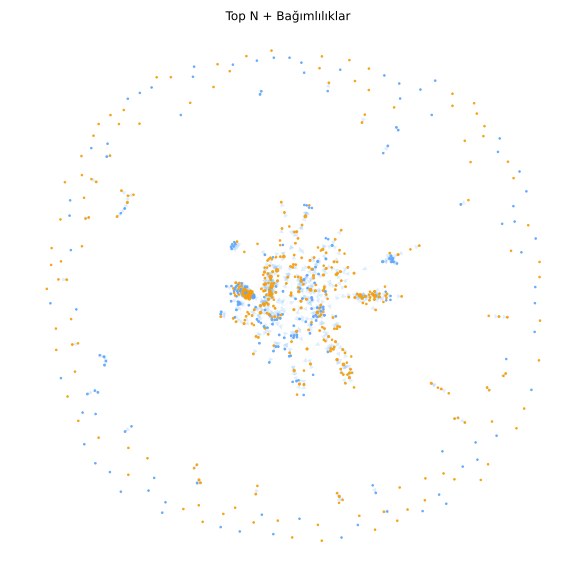
\includegraphics[width=\linewidth]{network_full_topN.png}
\caption{Visualization of the top 1000 package network. Dense regions indicate sub-clusters.}
\label{fig:network}
\end{figure}

\begin{figure}[H]
\centering
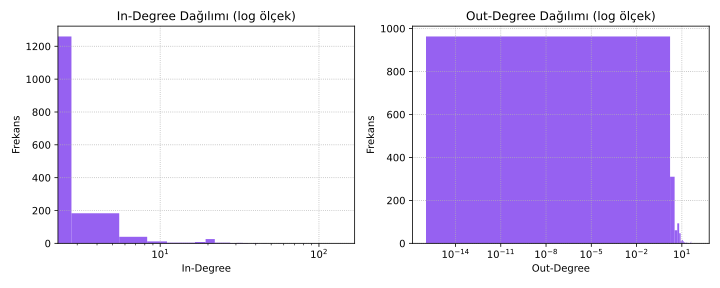
\includegraphics[width=\linewidth]{degree_histograms.png}
\caption{In-degree and out-degree histograms. The heavy-tailed structure of the distribution is visible.}
\label{fig:histograms}
\end{figure}

Figure \ref{fig:network} shows the clustering structure of the network topology. The degree distributions in Figure \ref{fig:histograms} indicate the scale-free structure of the network. While the majority of nodes have few connections, a small number of nodes have a high number of connections. This finding indicates that risk is concentrated in a specific section.

\subsection{Centrality Relationships}
\begin{figure}[H]
\centering
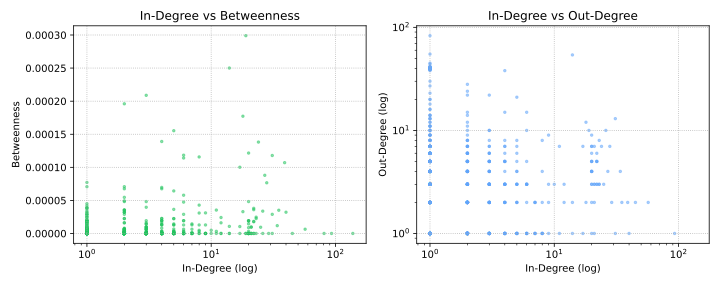
\includegraphics[width=\linewidth]{scatter_correlations.png}
\caption{Correlations between centrality measures.}
\label{fig:scatter}
\end{figure}

The correlation matrix (Figure \ref{fig:scatter}) shows an asymmetric relationship between in-degree and betweenness. It was determined that some packages without high popularity serve as bridges. It is evaluated that analyses focusing solely on download numbers may be insufficient in detecting structural risks.

\subsection{Analysis of Critical Nodes}
\begin{table}[H]
\centering
\caption{\textsc{Top 10 In-Degree}}
\label{tab:indegree}
\resizebox{\linewidth}{!}{%
\begin{tabular}{lrrrr}
\toprule
Package & In-Degree & Out-Degree & Betweenness & TopN? \\
\midrule
@babel/helper-plugin-utils & 110 & 0 & 0.000000 & True \\
call-bound & 41 & 2 & 0.000283 & False \\
postcss-value-parser & 39 & 0 & 0.000000 & True \\
call-bind & 36 & 4 & 0.000000 & False \\
@types/node & 34 & 1 & 0.000067 & False \\
debug & 34 & 1 & 0.000100 & True \\
es-errors & 33 & 0 & 0.000000 & False \\
@babel/types & 32 & 2 & 0.000236 & True \\
define-properties & 29 & 3 & 0.000000 & False \\
chalk & 28 & 0 & 0.000000 & False \\
\bottomrule
\end{tabular}%
}
\end{table}

\begin{table}[H]
\centering
\caption{\textsc{Top 10 Out-Degree}}
\label{tab:outdegree}
\resizebox{\linewidth}{!}{%
\begin{tabular}{lrrrr}
\toprule
Package & Out-Degree & In-Degree & Betweenness & TopN? \\
\midrule
@babel/preset-env & 70 & 3 & 0.000000 & True \\
postcss-preset-env & 67 & 1 & 0.000000 & True \\
es-abstract & 54 & 17 & 0.000000 & False \\
react-scripts & 48 & 0 & 0.000000 & True \\
workbox-build & 37 & 1 & 0.000000 & True \\
eslint & 34 & 1 & 0.000000 & True \\
cssnano-preset-default & 30 & 1 & 0.000000 & True \\
webpack-dev-server & 28 & 1 & 0.000000 & True \\
@jest/core & 28 & 2 & 0.000000 & True \\
express & 27 & 1 & 0.000000 & True \\
\bottomrule
\end{tabular}%
}
\end{table}

\begin{table}[H]
\centering
\caption{\textsc{Top 10 Betweenness}}
\label{tab:betweenness}
\resizebox{\linewidth}{!}{%
\begin{tabular}{lrrrr}
\toprule
Package & Betweenness & In-Degree & Out-Degree & TopN? \\
\midrule
jest-circus & 0.001144 & 1 & 20 & False \\
@babel/core & 0.001112 & 12 & 15 & True \\
babel-jest & 0.001087 & 2 & 7 & True \\
jest-runner & 0.001000 & 2 & 22 & True \\
@babel/helper-create-class-features-plugin & 0.000798 & 10 & 7 & True \\
get-intrinsic & 0.000771 & 22 & 10 & True \\
jest-snapshot & 0.000549 & 6 & 21 & True \\
@babel/traverse & 0.000523 & 20 & 7 & True \\
babel-preset-current-node-syntax & 0.000499 & 2 & 15 & False \\
babel-plugin-istanbul & 0.000466 & 2 & 5 & True \\
\bottomrule
\end{tabular}%
}
\end{table}

Packages with high in-degree in Table \ref{tab:indegree} are frequently used components. Packages with high out-degree in Table \ref{tab:outdegree} create a large attack surface. Table \ref{tab:betweenness} shows packages managing network traffic. For example, although the \texttt{jest-circus} package has a low in-degree (1), it assumes a critical bridge role in the network with a high betweenness value. Similarly, \texttt{@babel/core} stands out with both its popularity and strategic position. This situation proves that a single metric is not sufficient in risk analysis and the importance of detecting structural bridges.

\subsection{Composite Risk Score (BRS) Ranking}
\begin{figure}[H]
\centering
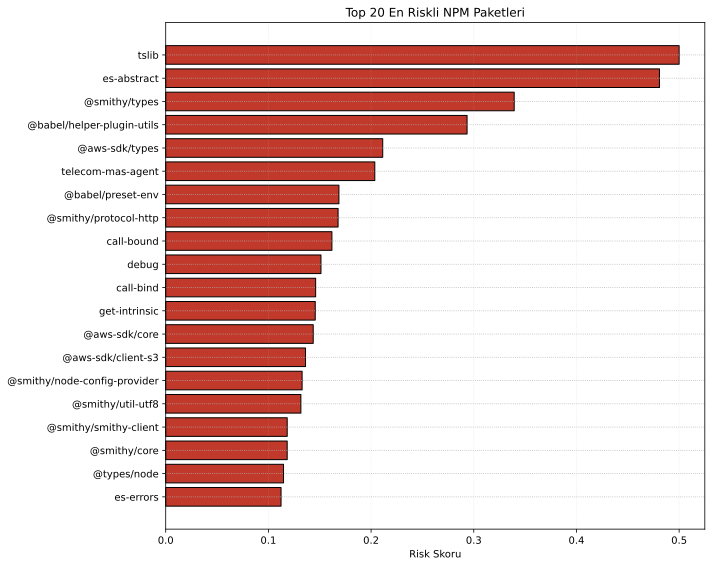
\includegraphics[width=\linewidth]{top20_risk_scores.png}
\caption{Top 20 packages with the highest Composite Risk Score (BRS).}
\label{fig:risk_scores}
\end{figure}

\begin{table}[H]
\centering
\caption{\textsc{Top 20 Composite Risk Score (BRS)}}
\label{tab:risk}
\resizebox{\linewidth}{!}{%
\begin{tabular}{lrrrrr}
\toprule
Package & Risk & In-Degree & Out-Degree & Betweenness & TopN? \\
\midrule
@babel/helper-plugin-utils & 0.500000 & 110 & 0 & 0.000000 & True \\
@babel/core & 0.388827 & 12 & 15 & 0.001112 & True \\
jest-circus & 0.361688 & 1 & 20 & 0.001144 & False \\
jest-runner & 0.334157 & 2 & 22 & 0.001000 & True \\
get-intrinsic & 0.330606 & 22 & 10 & 0.000771 & True \\
babel-jest & 0.313975 & 2 & 7 & 0.001087 & True \\
@babel/helper-create-class-features-plugin & 0.274757 & 10 & 7 & 0.000798 & True \\
call-bound & 0.266206 & 41 & 2 & 0.000283 & False \\
@babel/traverse & 0.248118 & 20 & 7 & 0.000523 & True \\
es-abstract & 0.231558 & 17 & 54 & 0.000000 & False \\
jest-snapshot & 0.231168 & 6 & 21 & 0.000549 & True \\
@babel/preset-env & 0.213636 & 3 & 70 & 0.000000 & True \\
@babel/types & 0.212942 & 32 & 2 & 0.000236 & True \\
postcss-preset-env & 0.195974 & 1 & 67 & 0.000000 & True \\
@jest/types & 0.193414 & 26 & 7 & 0.000211 & True \\
debug & 0.183565 & 34 & 1 & 0.000100 & True \\
babel-preset-current-node-syntax & 0.182762 & 2 & 15 & 0.000499 & False \\
postcss-value-parser & 0.177273 & 39 & 0 & 0.000000 & True \\
call-bind & 0.175065 & 36 & 4 & 0.000000 & False \\
@types/node & 0.174844 & 34 & 1 & 0.000067 & False \\
\bottomrule
\end{tabular}%
}
\end{table}
The BRS model combines popularity, attack surface, and strategic position. As seen in Figure \ref{fig:risk_scores} and Table \ref{tab:risk}, certain packages rank high due to both their popularity and network position. The ranking indicates packages to be prioritized in security audits.

\subsection{Systemic Impact and Cascade Analysis}
\begin{figure}[H]
\centering
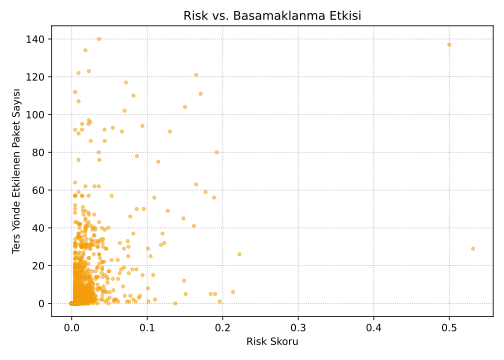
\includegraphics[width=\linewidth]{risk_vs_cascade.png}
\caption{Relationship between BRS and cascade effect (reachability).}
\label{fig:cascade}
\end{figure}

\begin{figure}[H]
\centering
\includegraphics[width=\linewidth]{top20_cascade_impact.png}
\caption{Impact of removing the top 20 packages on LCC and reachability.}
\label{fig:impact}
\end{figure}
Simulation results support the BRS model. In Figure \ref{fig:impact}, it is seen that the removal of packages with high BRS scores causes a decrease in LCC size. The correlation between BRS score and cascade effect (Figure \ref{fig:cascade}) demonstrates the metric's success in risk prediction.

\section{Discussion and Conclusion}
In this study, moving beyond descriptive analyses in the literature, a \textbf{Composite Risk Score (BRS)} model that converts structural risks in the NPM ecosystem into a measurable value is presented. The lack of "operational prioritization" mentioned in the introduction has been addressed with the obtained BRS ranking. Analyses have shown that the security of the network depends not only on popular packages but also on infrastructural bridge packages like \texttt{jest-circus} or \texttt{@babel/core}. The findings confirm the "small-world" network structure stated by Zimmermann et al. \cite{zimmermann2019smallworld}; however, it expands the literature by revealing that risk is concentrated not only in popular packages but also in intermediate layer packages acting as bridges.

> **Scope of Impact Analysis**
>
> In this study, "Cascade Impact" simulations were performed on the constructed **"Critical Backbone Graph"** rather than the entire NPM registry, due to computational complexity and data access constraints. This approach relies on the "Supply Chain Backbone" hypothesis: The topological disintegration (loss of LCC) of this dense network, composed of critical infrastructure packages, serves as a reliable mathematical proxy for the functional failure of millions of dependent projects. Therefore, the structural collapse of the local backbone is interpreted as a direct indicator of global systemic risk.

\subsection{Limitations of the Study}
The analysis is limited to static dependencies defined in \texttt{package.json} files. Dynamically loaded packages at runtime or developer reputation are excluded from the scope at this stage. Additionally, the analysis was performed on an instantaneous snapshot and does not include the temporal evolution of the network. Similarly, legal risks such as license compliance \cite{ahlstrom2025licensing} are outside the scope of this study.

\subsection{Recommendations}
Based on the findings, the following recommendations have been developed:
\begin{itemize}
    \item \textbf{Prioritization:} Directing resources to packages with high BRS scores in security scans.
    \item \textbf{Policy Development:} Applying security protocols \cite{torres2020intoto} and SBOM practices \cite{yu2024sbom} to critical nodes.
    \item \textbf{Awareness:} Informing package owners about risk scores.
\end{itemize}

It is recommended to expand the model to include developer networks in future studies.

\section{Reproducibility}
Source codes and datasets have been shared for the reproducibility of the study:
\begin{itemize}
  \item \textbf{Analysis Codes:} \texttt{analysis/analysis.ipynb} (Python 3, NetworkX, pandas).
  \item \textbf{Data Outputs:} All intermediate results and metrics are presented in CSV/JSON format in the \texttt{results/} directory.
\end{itemize}

\bibliographystyle{IEEEtran}
\bibliography{bib}

\end{document}
